\documentclass[12pt]{article}
\usepackage{graphicx, subfigure, float, amsmath, amssymb, color}
\usepackage[margin = 1.0 in]{geometry}
\usepackage{natbib}

\renewcommand{\bottomfraction}{.9}
\renewcommand{\topfraction}{.9}
\renewcommand{\textfraction}{0.1}
\renewcommand{\floatpagefraction}{.9}



% definition of \customlabel, which is used to label supplementary figures and tables
\makeatletter
\newcommand{\customlabel}[2]{%
\protected@write \@auxout {}{\string \newlabel {#1}{{#2}{}}}}
\makeatother


%\title{}
\title{Amino-acid site variability among natural and designed proteins}
\author{Eleisha L.\ Jackson, Noah Ollikainen, Arthur W.\ Covert III,\\ Tanja Kortemme, and Claus O.\ Wilke}
\begin{document}

\date{}
\maketitle

\section*{Supporting Figures}

\centerline{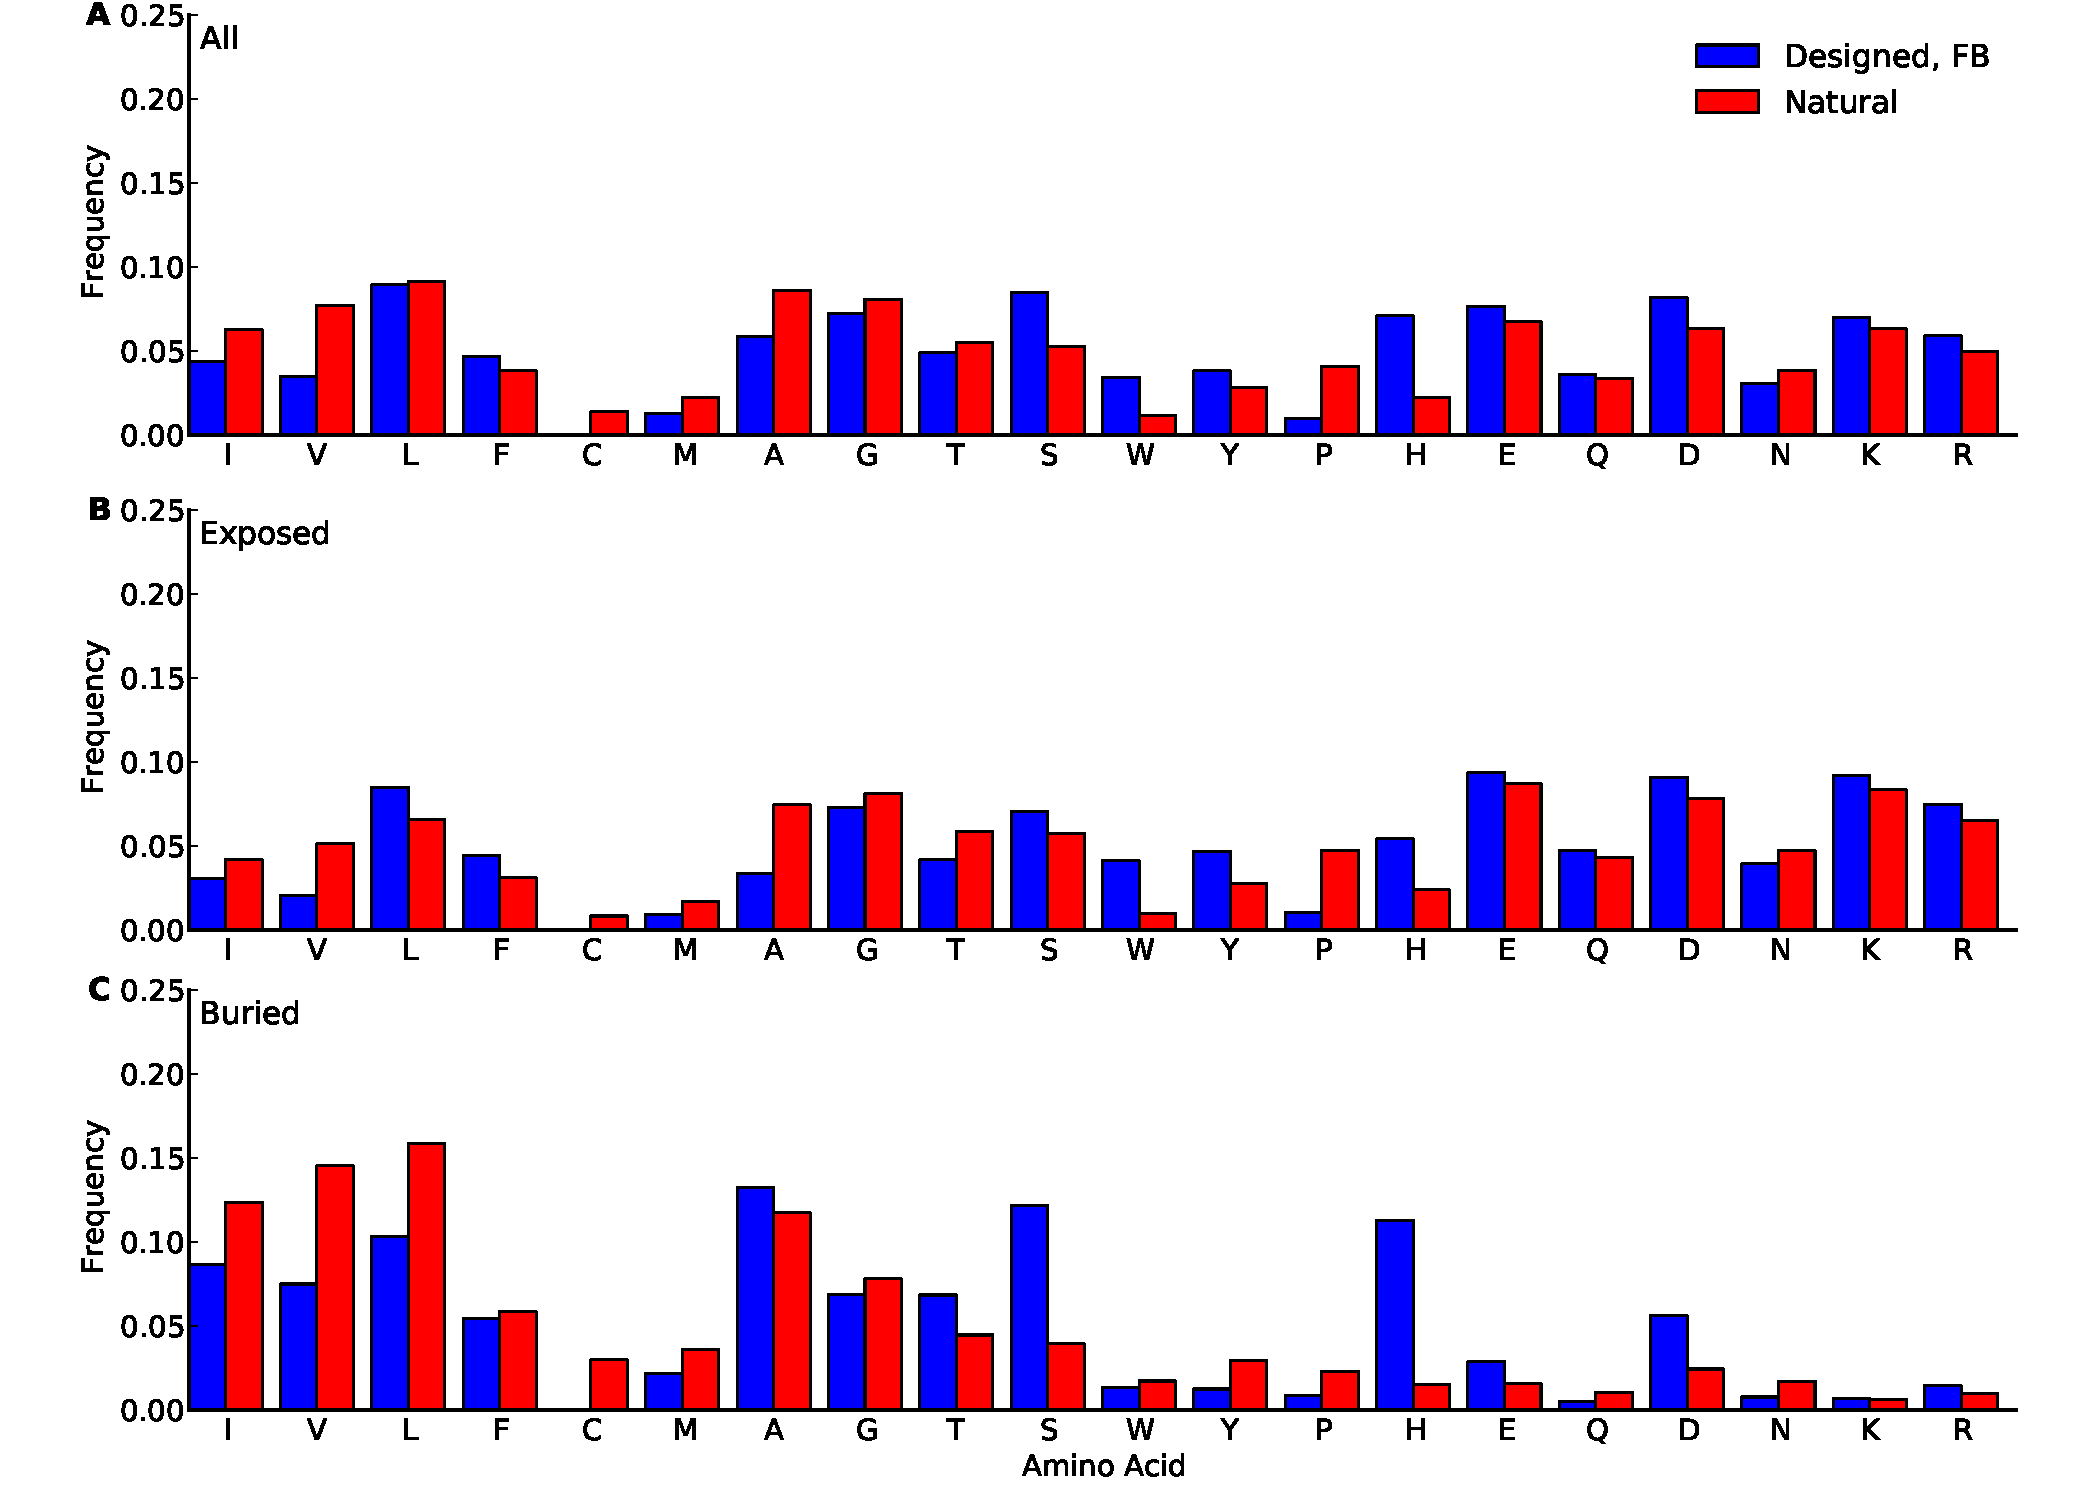
\includegraphics[width = 5in]{figures/Duncan_Freq_Combo_Plots_00.pdf}}

\noindent Figure S1. Amino-acid frequencies in designed and natural proteins. Frequencies were calculated over all sites in all proteins belonging to the yeast-proteins data set. For designed proteins, only fixed-backbone designs were considered. Top: overall frequencies. Middle: frequencies at exposed sites (defined as sites with $\text{RSA}>0.05$). Bottom: frequencies at buried sites (defined as sites with $\text{RSA}\leq0.05$).

\customlabel{AAFreqsYeastProteins00}{S1}


\newpage

\centerline{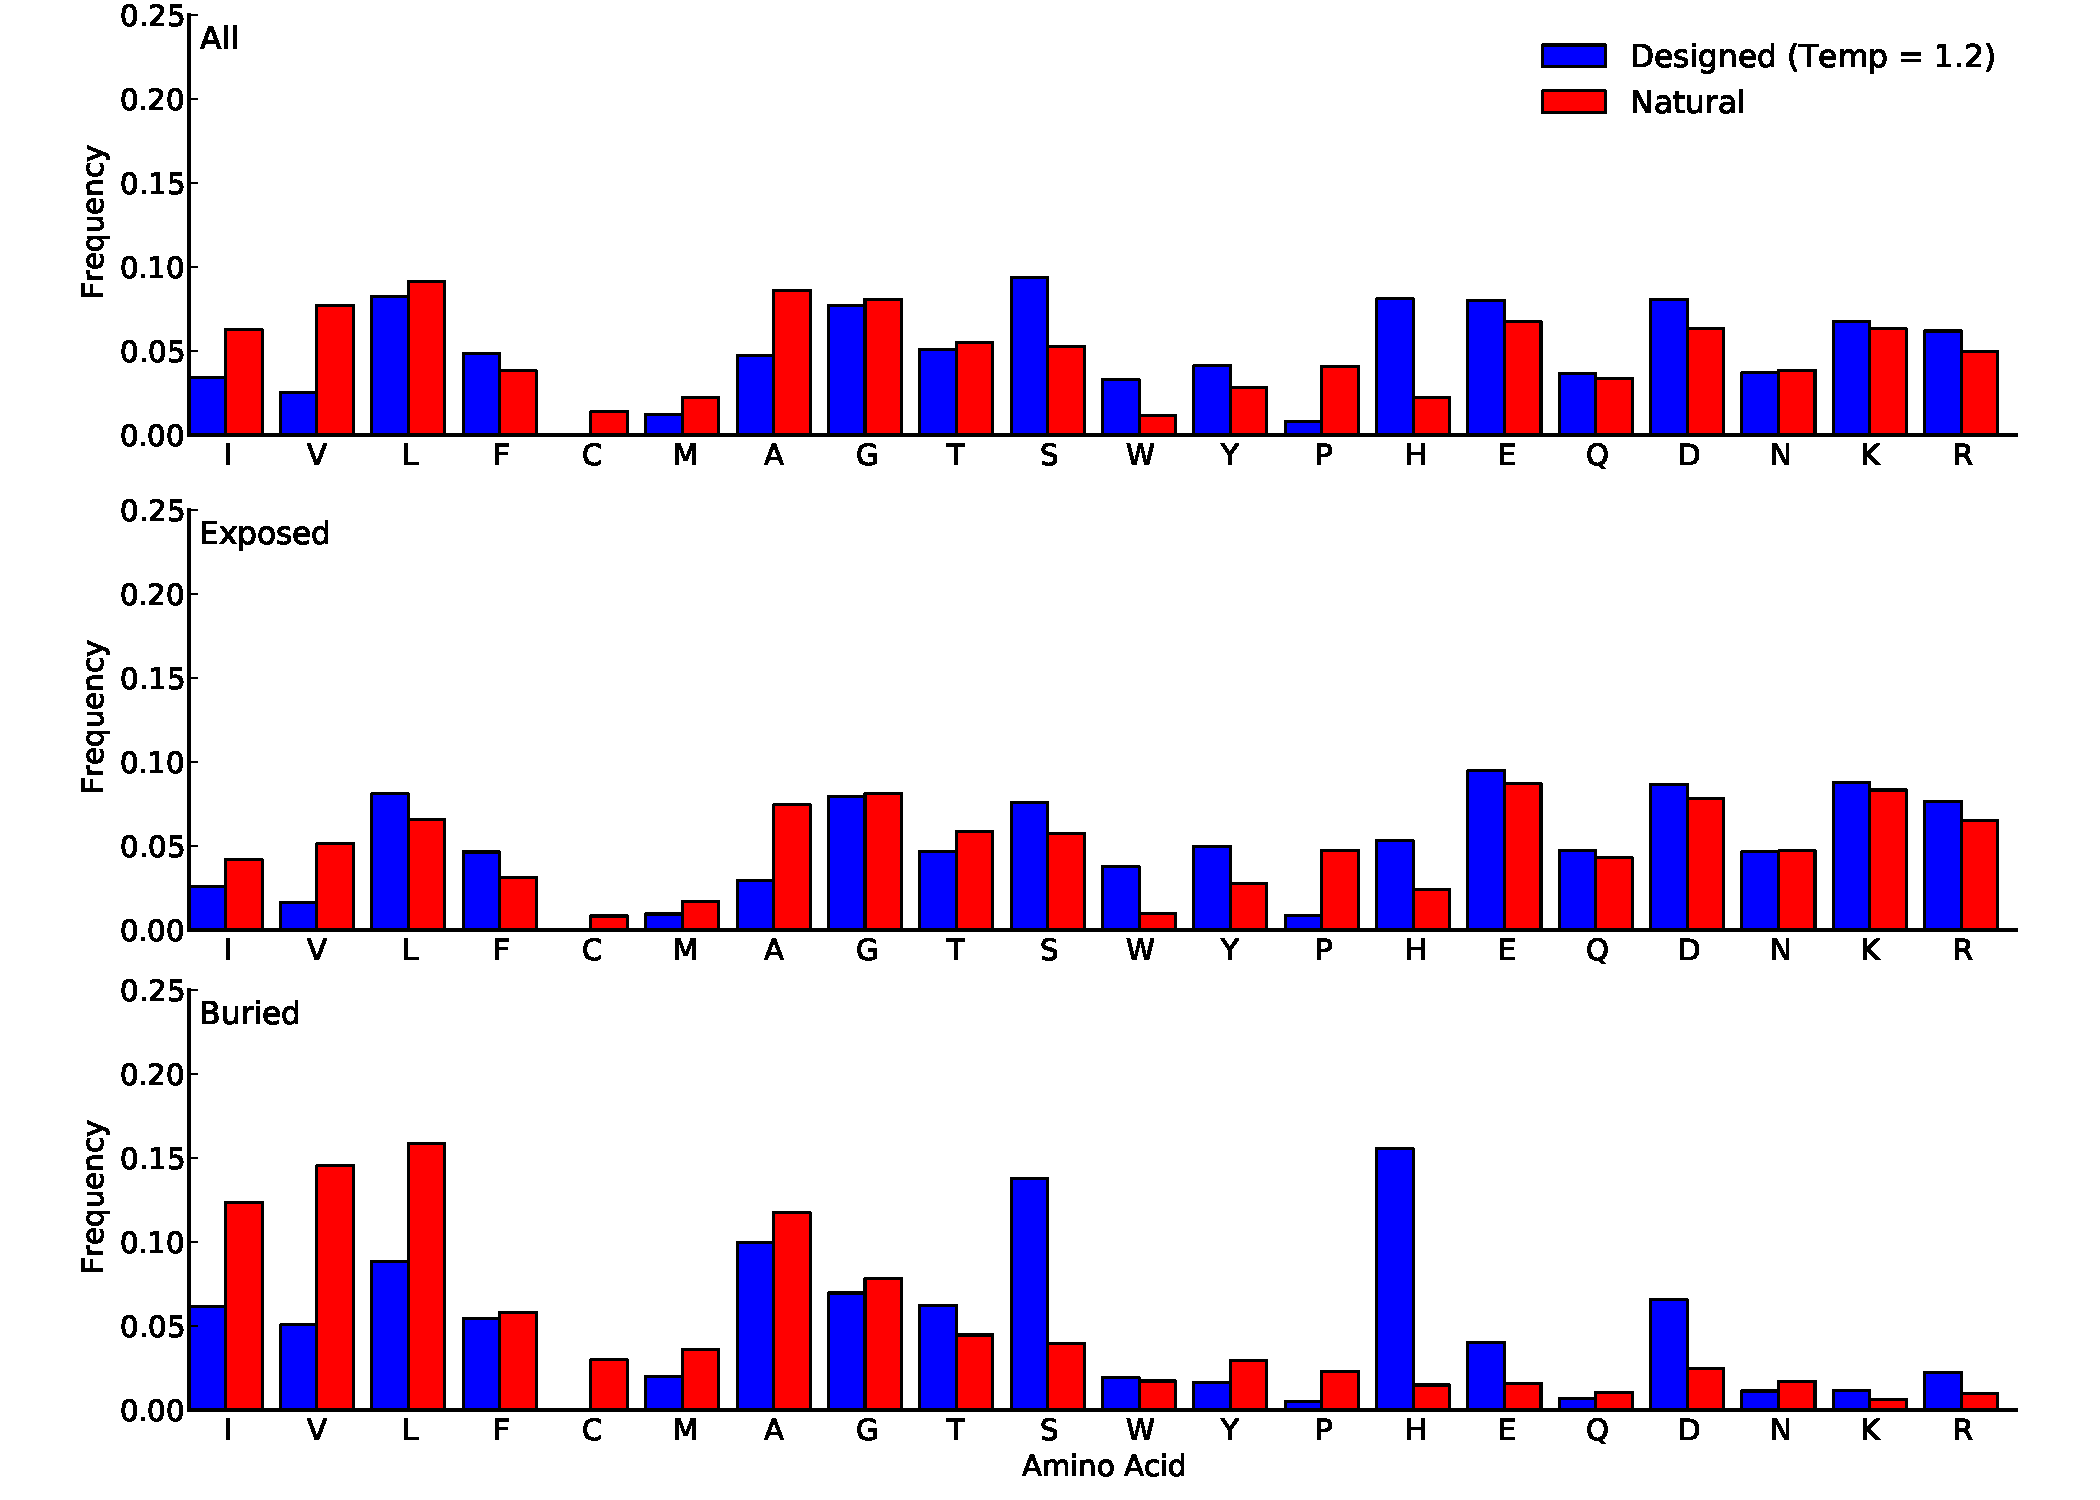
\includegraphics[width = 5in]{figures/Duncan_Freq_Combo_Plots_12.pdf}}

\noindent Figure S2. Amino-acid frequencies in designed and natural proteins. Frequencies were calculated over all sites in all proteins belonging to the yeast-proteins data set. For designed proteins, only flexible-backbone designs with design temperature 1.2 were considered. Top: overall frequencies. Middle: frequencies at exposed sites (defined as sites with $\text{RSA}>0.05$). Bottom: frequencies at buried sites (defined as sites with $\text{RSA}\leq0.05$).

\customlabel{AAFreqsYeastProteins12}{S2}

\newpage

\centerline{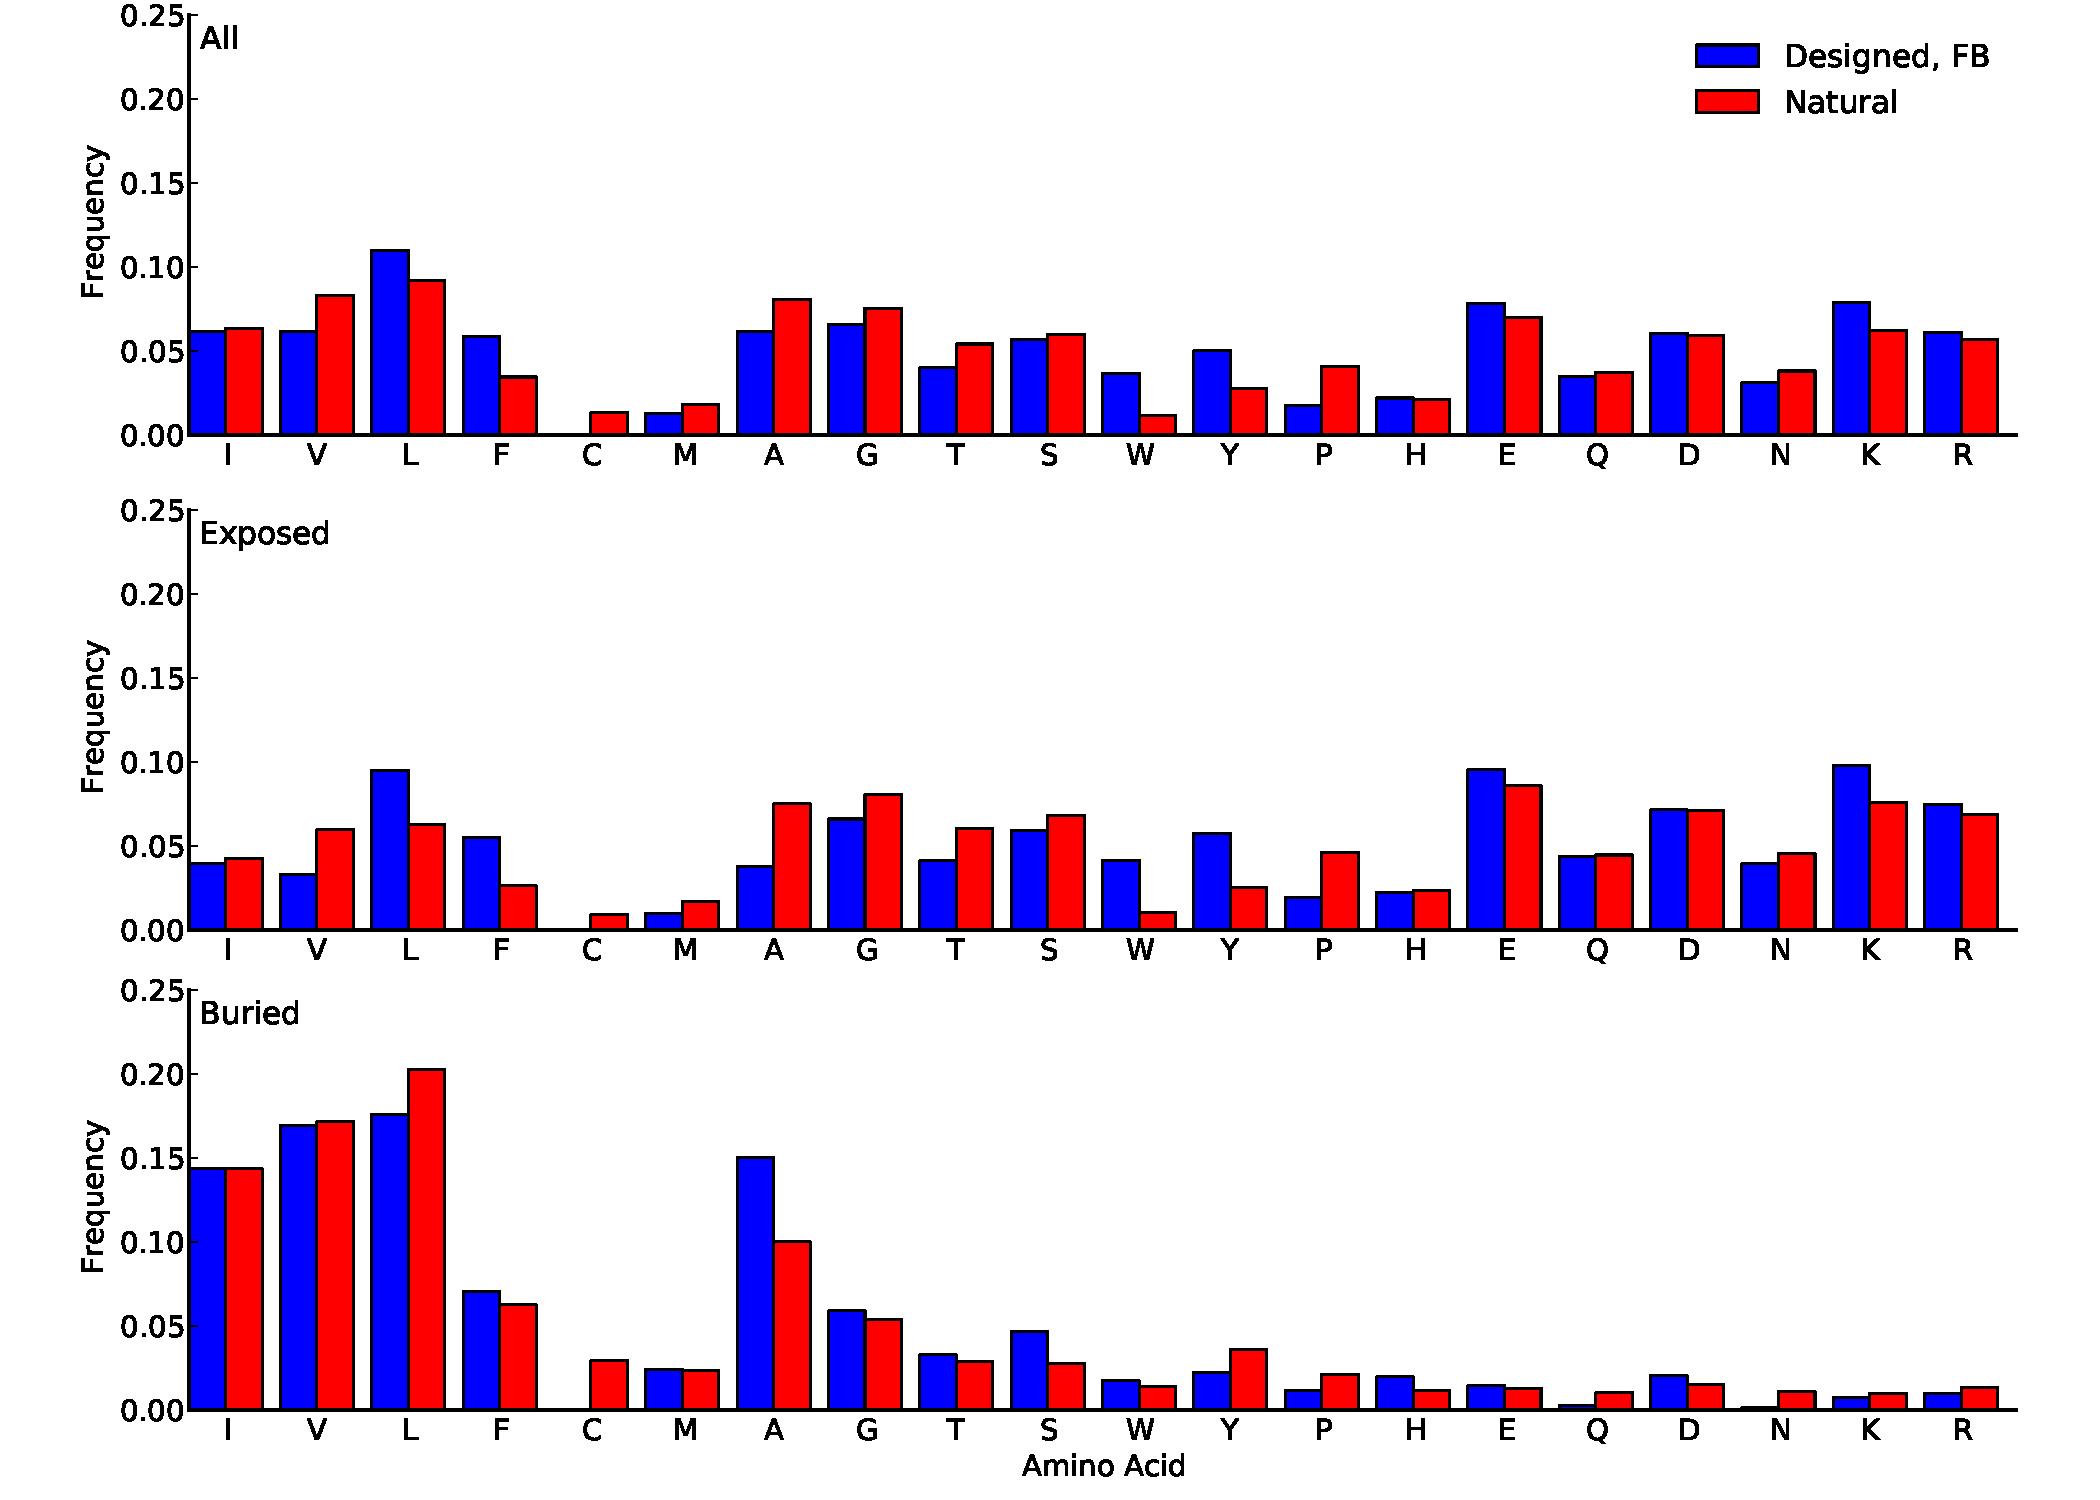
\includegraphics[width = 5in]{figures/Noah_Freq_Combo_Plots_00.pdf}}

\noindent Figure S3. Amino-acid frequencies in designed and natural proteins. Frequencies were calculated over all sites in all proteins belonging to the protein-domains data set. For designed proteins, only fixed-backbone designs were considered. Top: overall frequencies. Middle: frequencies at exposed sites (defined as sites with $\text{RSA}>0.05$). Bottom: frequencies at buried sites (defined as sites with $\text{RSA}\leq0.05$). 

\customlabel{AAFreqsProteinDomains00}{S3}

\newpage

\centerline{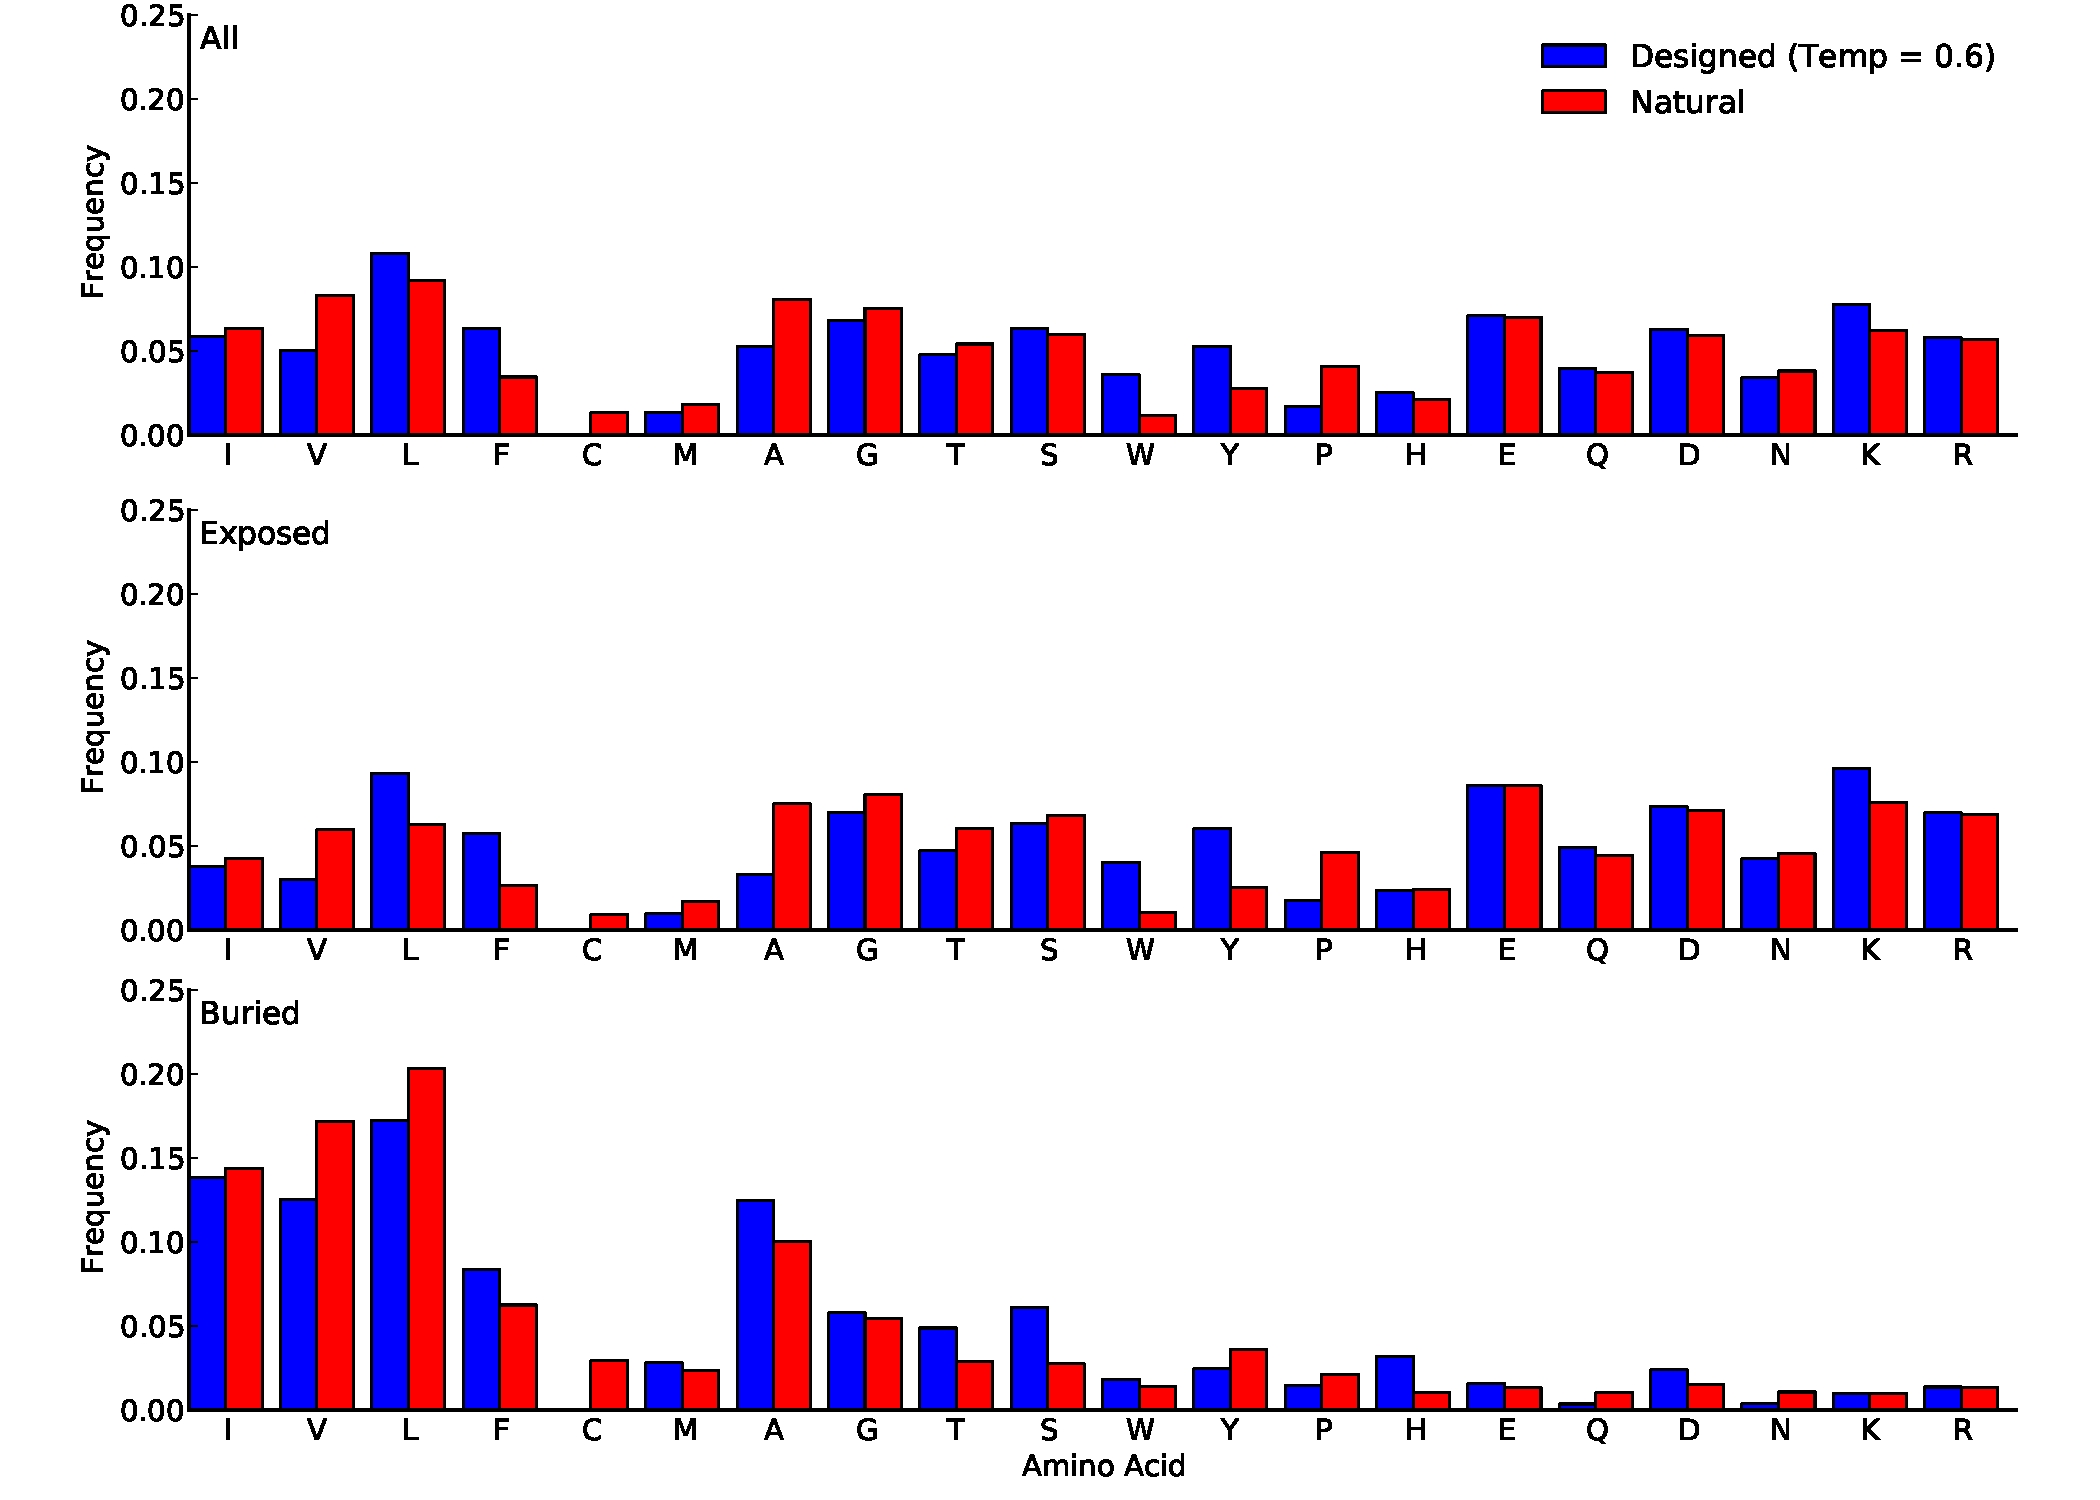
\includegraphics[width = 5in]{figures/Noah_Freq_Combo_Plots_06.pdf}}

\noindent Figure S4. Amino-acid frequencies in designed and natural proteins. Frequencies were calculated over all sites in all proteins belonging to the protein-domains data set. For designed proteins, only flexible-backbone designs with design temperature 0.6 were considered. Top: overall frequencies. Middle: frequencies at exposed sites (defined as sites with $\text{RSA}>0.05$). Bottom: frequencies at buried sites (defined as sites with $\text{RSA}\leq0.05$). 

\customlabel{AAFreqsProteinDomains06}{S4}

\newpage

\centerline{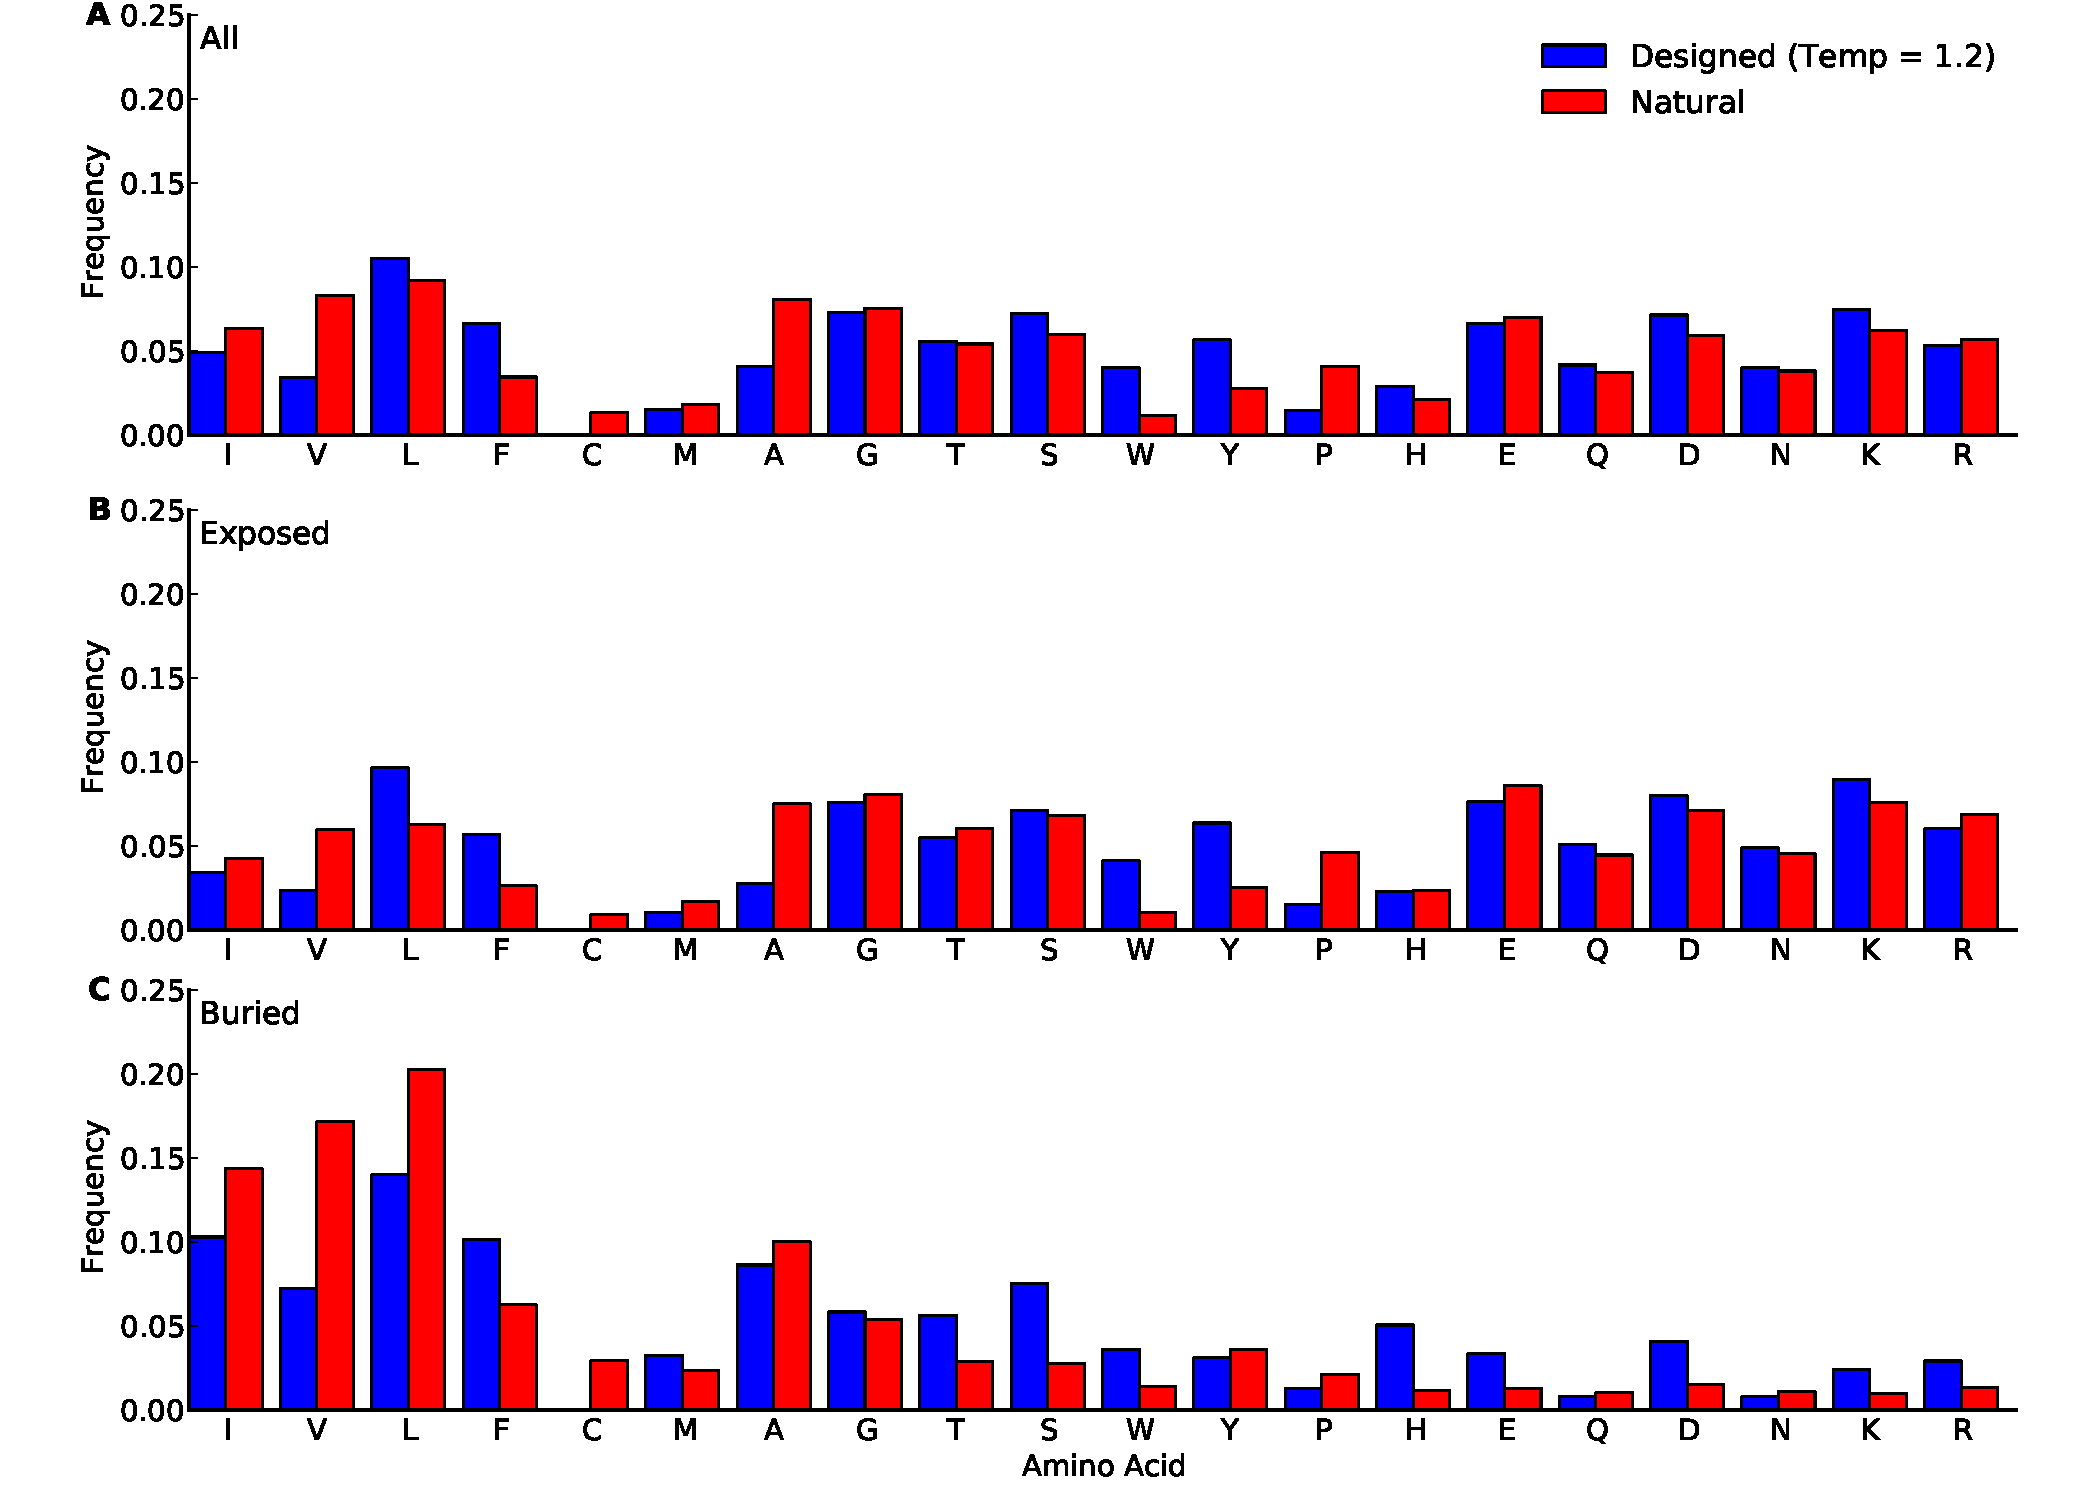
\includegraphics[width = 5in]{figures/Noah_Freq_Combo_Plots_12.pdf}}

\noindent Figure S5. Amino-acid frequencies in designed and natural proteins. Frequencies were calculated over all sites in all proteins belonging to the protein-domains data set. For designed proteins, only flexible-backbone designs with design temperature 1.2 were considered. Top: overall frequencies. Middle: frequencies at exposed sites (defined as sites with $\text{RSA}>0.05$). Bottom: frequencies at buried sites (defined as sites with $\text{RSA}\leq0.05$). 

\customlabel{AAFreqsProteinDomains12}{S5}


\newpage

\centerline{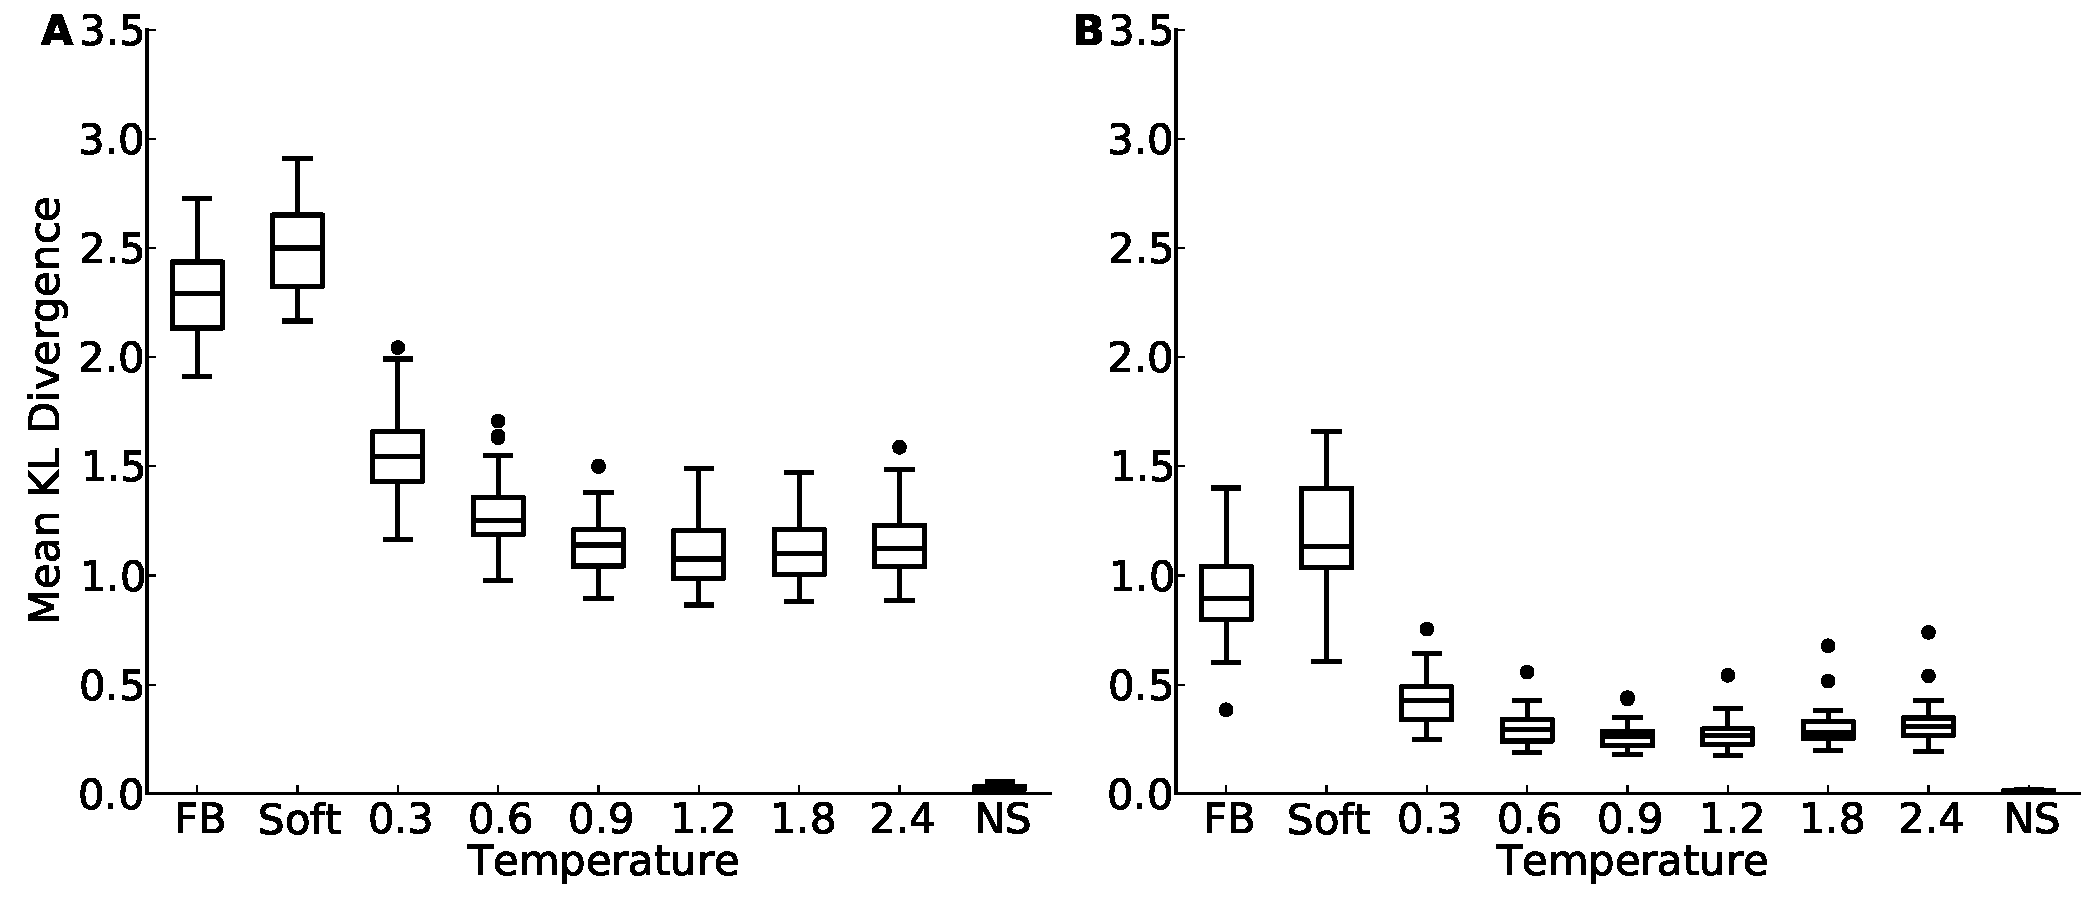
\includegraphics[width = 6in]{figures/Mean_KL_vs_Temp_Boxplot_Noah.pdf}}

\noindent Figure S6. Mean Kullback-Leibler (KL) divergence for designed and natural proteins, shown for the yeast-proteins data set. A higher KL divergence indicates that the amino-acid distributions at sites in designed proteins are less similar to the corresponding distributions in the natural proteins. ``FB'' refers to fixed backbone design, and ``NS'' refers to the control case where natural sequences are compared to themselves. (A) KL divergence calculated from the relative frequencies of the 20 amino acids. (B) KL divergence calculated from rank-ordered frequency distributions. The most common amino acid in the reference distribution is compared to the most common amino acid in the focal distribution, the same is done for the second-most common amino acid, and so on, irrespective of the type of amino acids.

\customlabel{NoahAADisFig1}{S6}

\newpage


\centerline{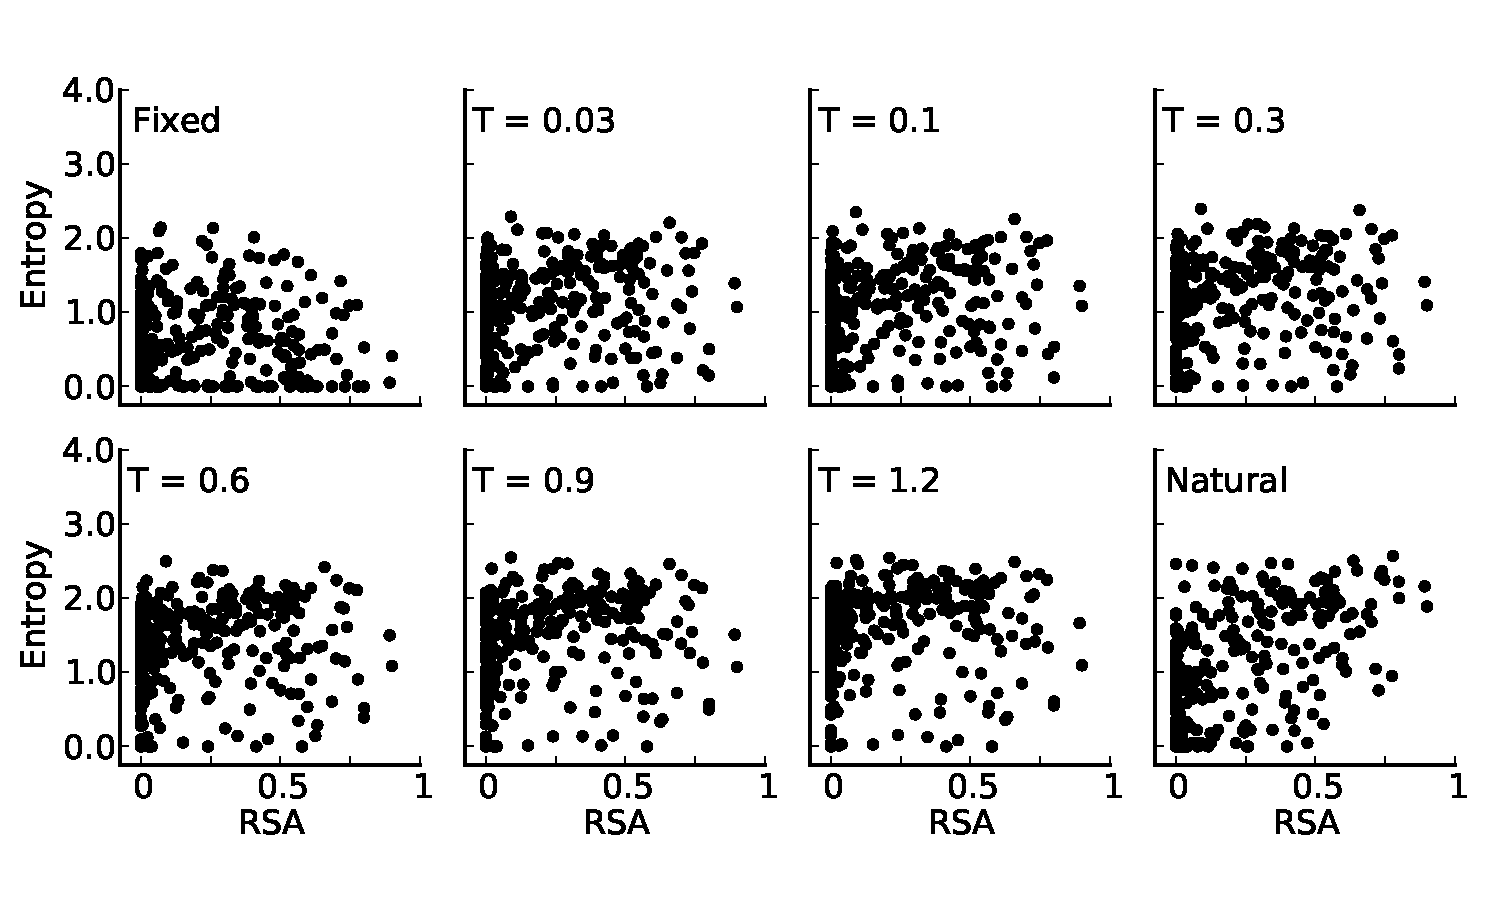
\includegraphics[width = 6.5in]{figures/RSA_vs_Entropy_1PV1_Combination_Plot.pdf}}

\noindent Figure S7. Site entropy versus Relative Solvent Accessibility (RSA) for designed and natural sequence alignments of the protein S-formylglutathione hydrolase (PDB: 1PV1, chain A).  Natural sequences exhibit a clear trend of higher site variability at higher RSA values. The flexible backbone designs exhibit a similar trend but the fixed backbone designs do not.
\customlabel{Entropy_vs_RSA_example}{S7}

\newpage

\centerline{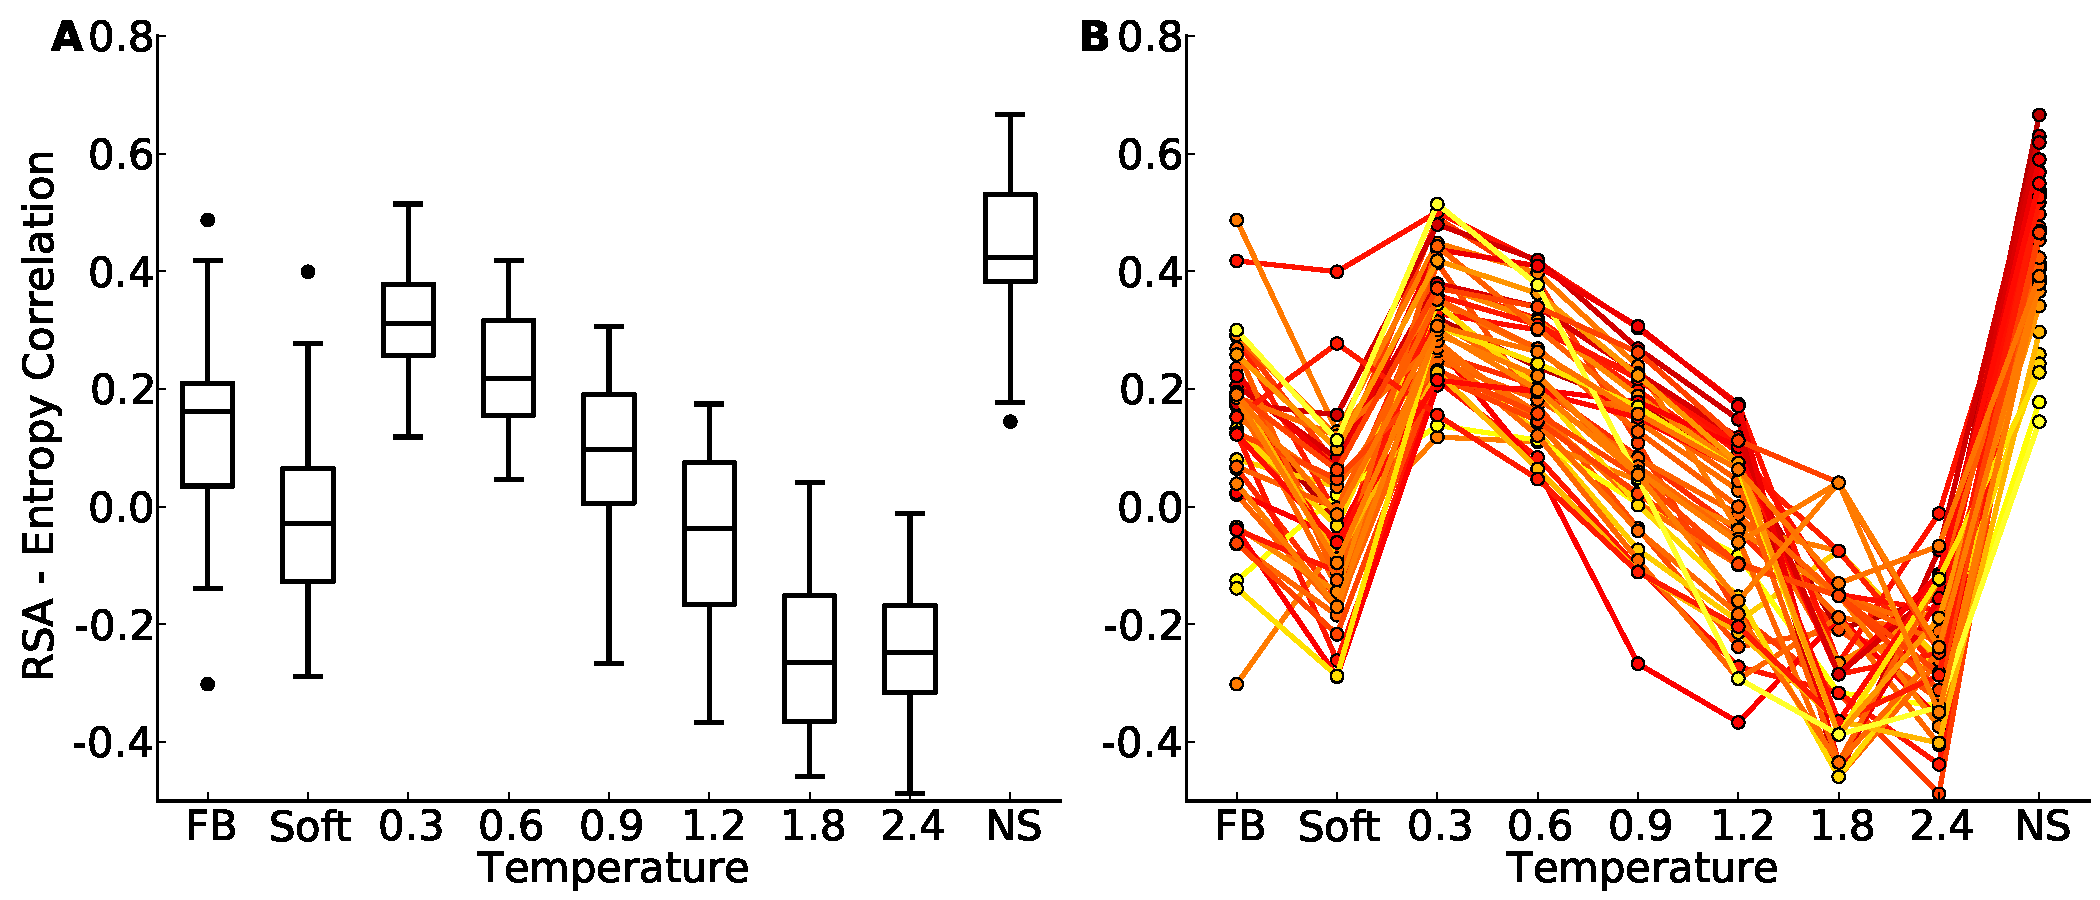
\includegraphics[width = 6in]{figures/Cor_Mean_Entropy_RSA_Combination_Plot_Noah.pdf}}
\noindent Figure S8. Distributions of correlation coefficients between site entropy and RSA, for the yeast-proteins data set. ``FB'' indicates fixed-backbone design, ``Soft'' indicates soft backbone design, and ``NS'' indicates natural sequences. (A) Distributions represented as boxplots. (B) Correlation coefficients for individual proteins. Lines connect identical structures in the different design conditions. The color shading represents the strength of the correlation for the natural sequence alignment. In general, natural proteins display a stronger correlation between site entropy and RSA than designed proteins.

\customlabel{Correlation_figure_Noah}{S8}

\newpage

% \centerline{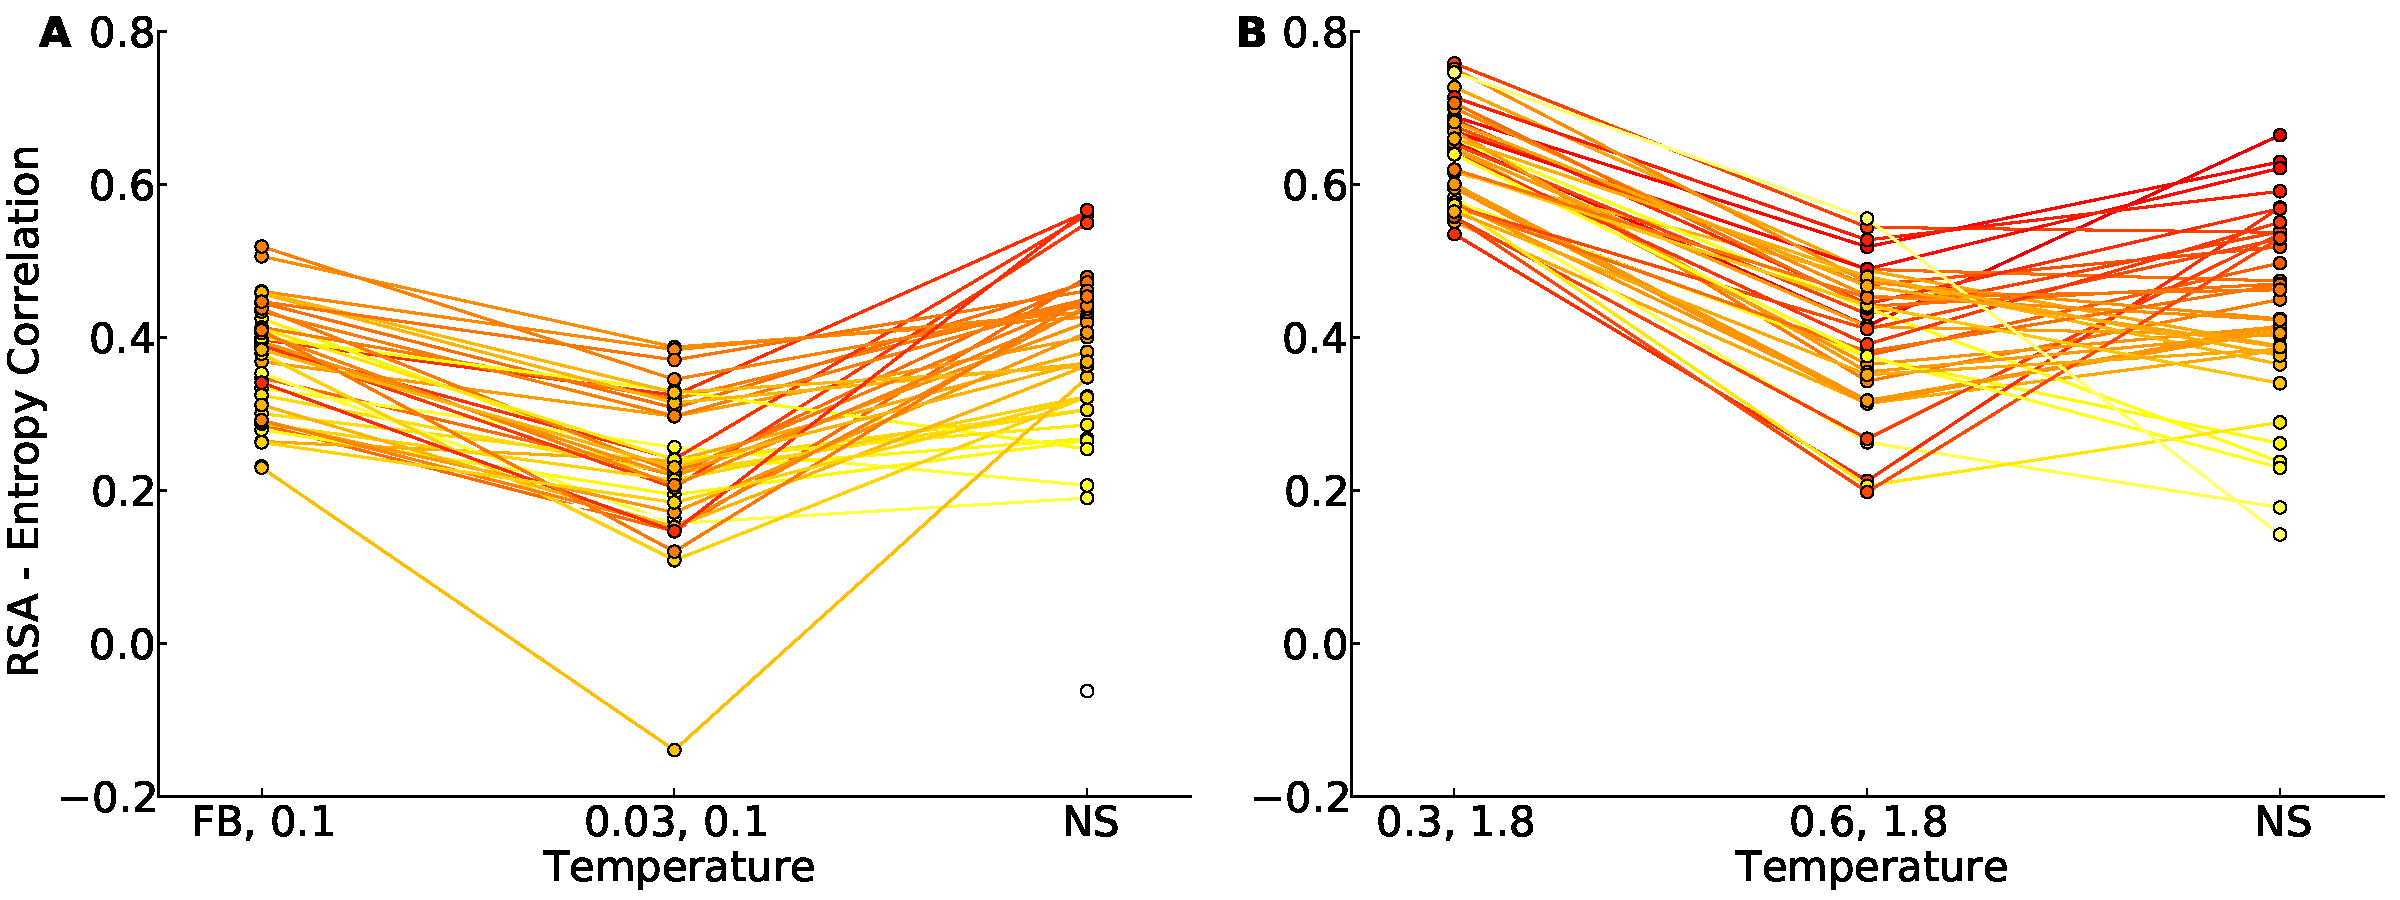
\includegraphics[width = 6in]{figures/Combo_Lineplot_Mixed_Temp_Correlation_Plot.pdf}}
% \noindent Figure S4.  Distribution of  the correlation coefficients between RSA and site entropy for hybrid designed and natural proteins. Colors correspond to the magnitude of the correlation coefficient in the natural proteins. Hybrids were created by taking sequences for buried residues and partially residues from one temperature and exposed residues from another temperature (left: yeast proteins, right: protein domains). "NS" refers to the natural sequences and "FB" refers to fixed backbone. 
% \customlabel{Combo_Mixed_Entropy_Lineplot}{S5}
% 
% \newpage


\centerline{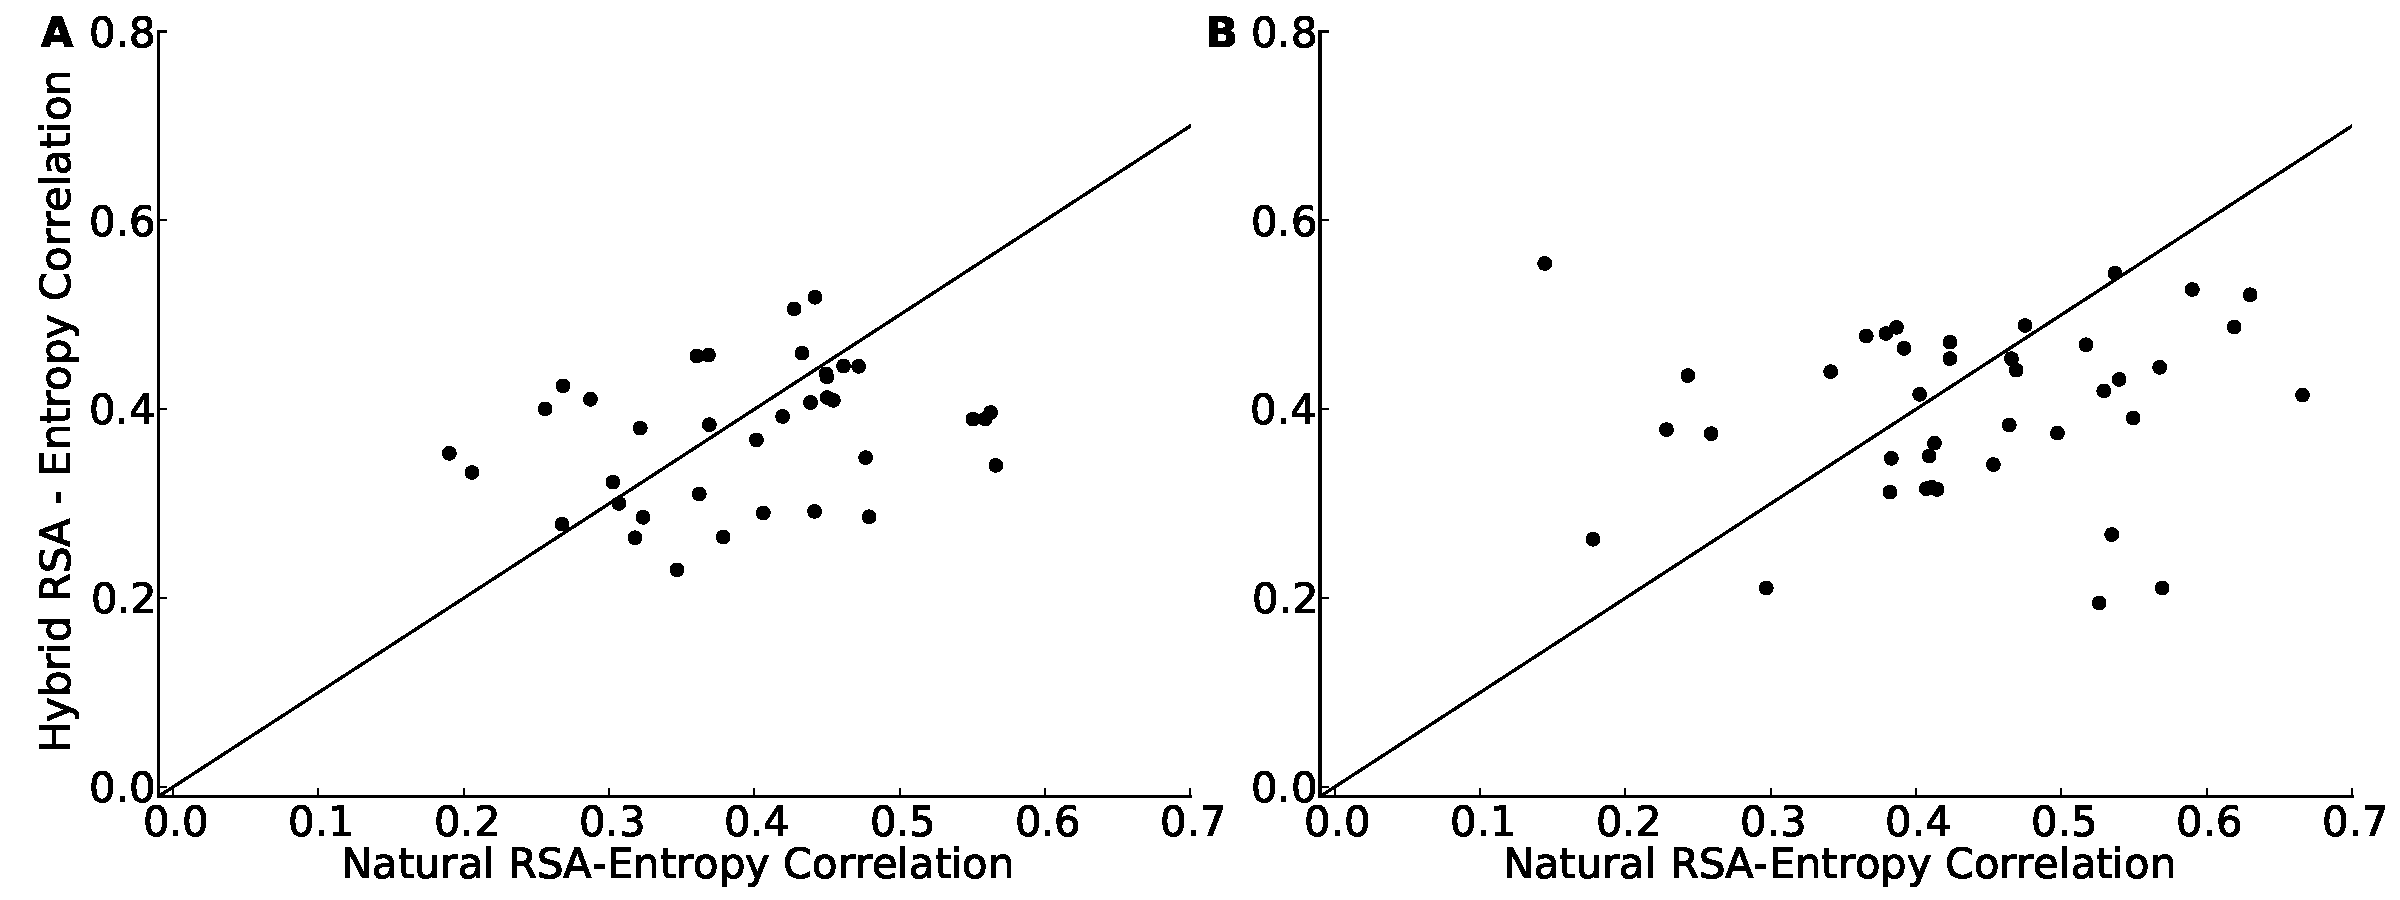
\includegraphics[width = 6in]{figures/Combo_Lineplot_Mixed_Temp_Correlation_Lineplot.pdf}}
\noindent Figure S9. Correlation coefficients between RSA and site entropy for hybrid designs and natural proteins. For the hybrid designs, buried and partially buried sites were taken from proteins designed with a fixed backbone (yeast proteins) or a temperature of $T = 0.6$ (protein domains). Exposed residues were taken from proteins designed with a temperature of $ T =  0.1$ (yeast proteins) or $T = 1.8$ (protein domains). The solid line indicates $y=x$. Note that while the range of correlation values in hybrid designs generally matches the range of values in natural alignments, predictions for specific proteins are not that accurate.

\customlabel{Mixed_Entropy_Correlation_Plot}{S9}

\end{document}